Nástrojů jak dnes psát dokumenty máme celou řadu, některé jsou volně dostupné a jiné jsou zpoplatněny. Některé nástroje jsme si již představili (Word, LibreOffice), ale
nyní se zaměříme na takzvané značkovací jazyky. Značkovací jazyky nám umožnují psát text, který je poté možné zpracovat počítačem, který změní jeho formátování. Většina
značkovacích jazyků má jasně rozlišitelné značky, nebo jinak také tagy, které upravují formátování při jejich strojovém překladu, díky tomu je původní text stále dobře čitelný.
\cite{markup}

Mezi značkovací jazyky například patří i jazyky používané při psaní webových stránek, jako je HTML či XML, ovšem tyto jazyky budeme spíše využívat pro zobrazování výstupu
jednodušších značkovacích jazyků jako je například Markdown.

\section{Markdown}

Markdown je značkovací jazyk, který převádí text do HTML. Jedná se o jednoduše čitelný a zároveň jednoduchý jazyk na psaní strukturovaného textu. Hlavní myšlenkou Markdown je, že
text v něm psaný by měl být publikovatelný i bez jeho zpracování, inspirací tomuto přístupu jsou čistě textové emaily (emaily se dnes ve většině případů píšou v HTML
z důvodu grafického obsahu). \cite{markdown}

\todo{Místa kde se markdown používá}

Takto vypadá menší ukázka Markdown syntaxe a také výsledek, který je poté generován.

\clearpage

\begin{minted}{md}
    # Ukázkový příklad Markdown syntaxe

    Takto vypadá dokument psaný v Markdown,
    jak je vidět, od čistého textu se moc neliší.

    ## Víceúrovňové nadpisy

    *kurzíva*, **tučné**, ~~přeskrtnuní~~

    - příklad
    - jednoduchého
    - seznamu

    - [ ] Checkbox
\end{minted}

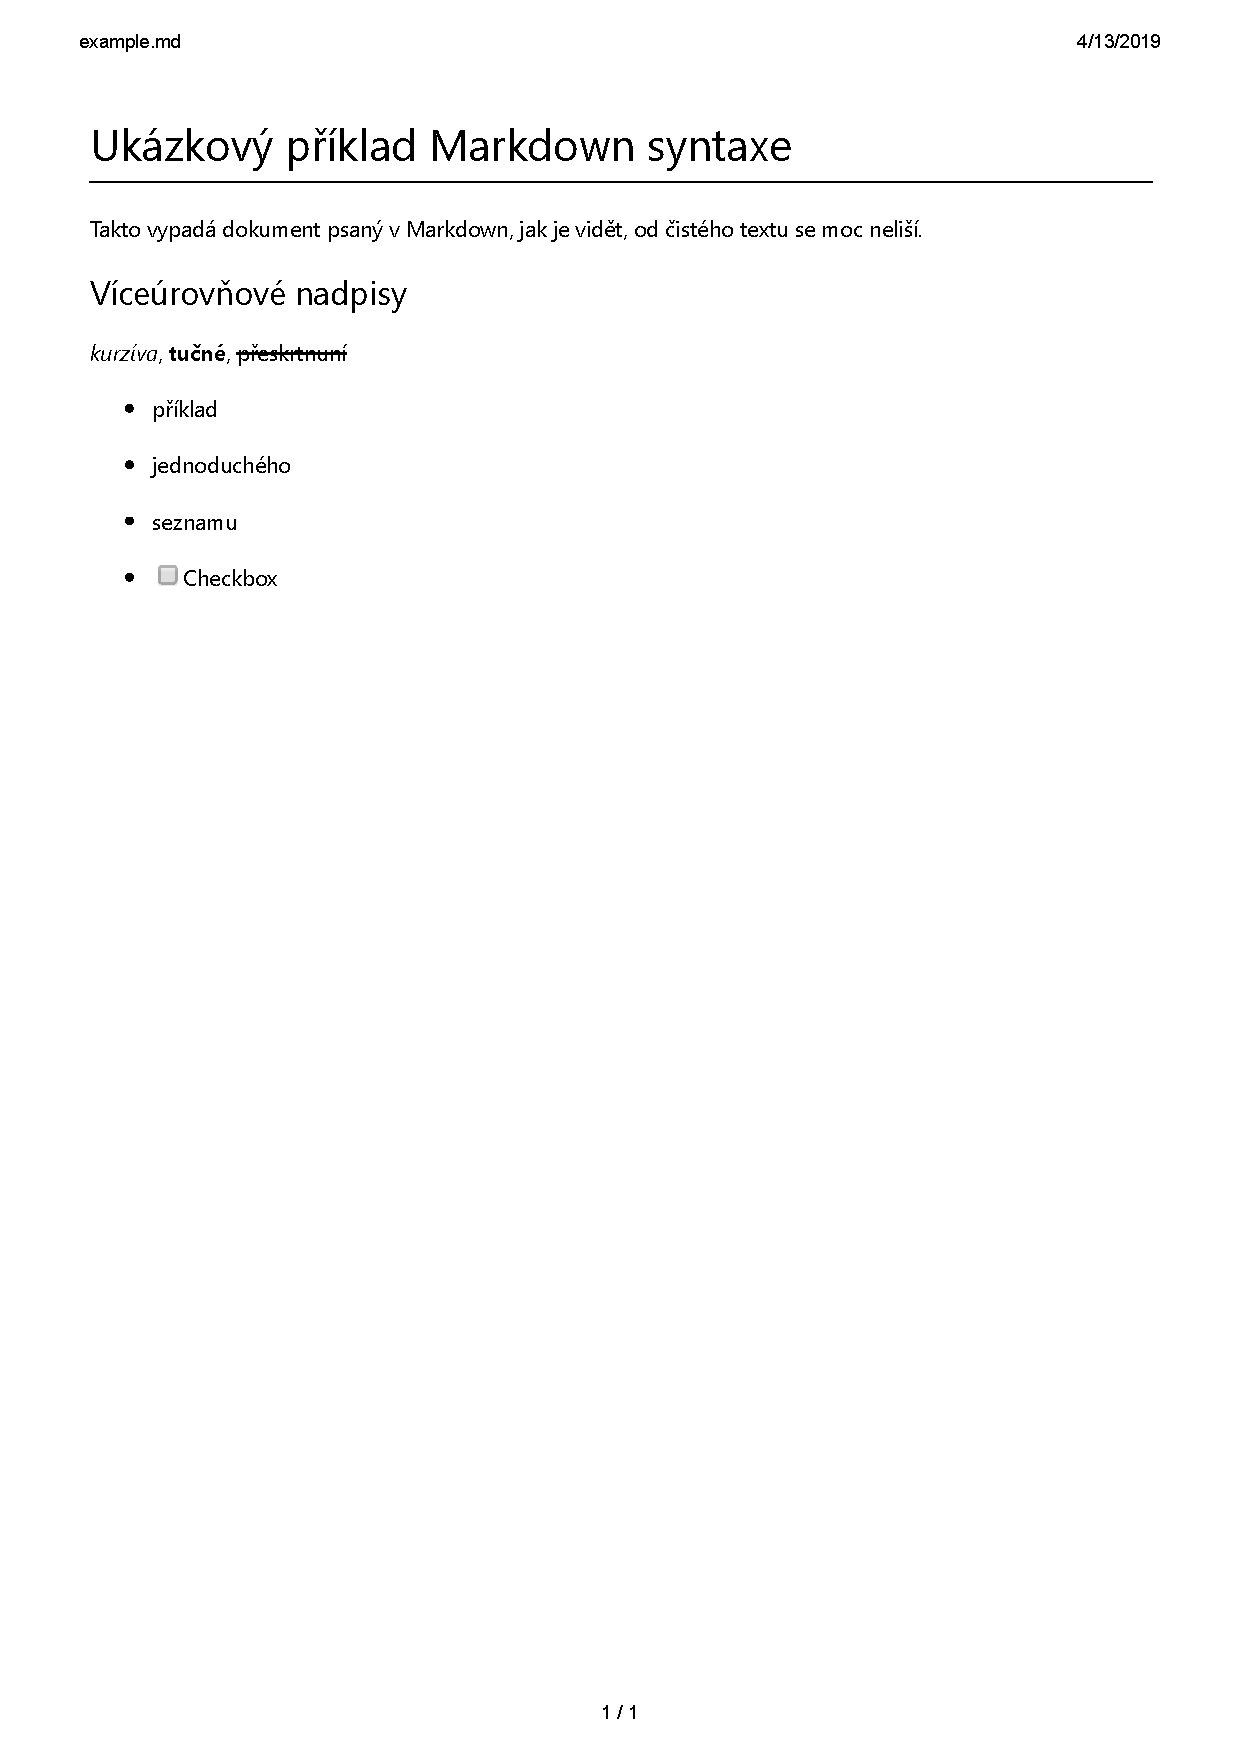
\includepdf{example.pdf}

\section{reStructuredText}

Formát reStructuredText pro psaní dokumentů v prostém textu, který je jednoduchý na čtení, kde je hned zřejmé jak bude vygenerovaný text vypadat.
Tento formát je jednoduchý na použití hlavně pro psaní programátorské dokumentace, jednoduchých webů a samostatných dokumentů.
Hlavním cílem reStructuredText je definovat a uplatnit jednoduchý značkovací jazyk pro použítí v Python, kde se používá k dokumentaci jednotlivých částí programu,
a dalších dokumentačních nástrojích, který je jednoduše čitelný a jednoduše použitelný. \cite{reStruDoc}

\inputminted{rst}{example-rst.rst}

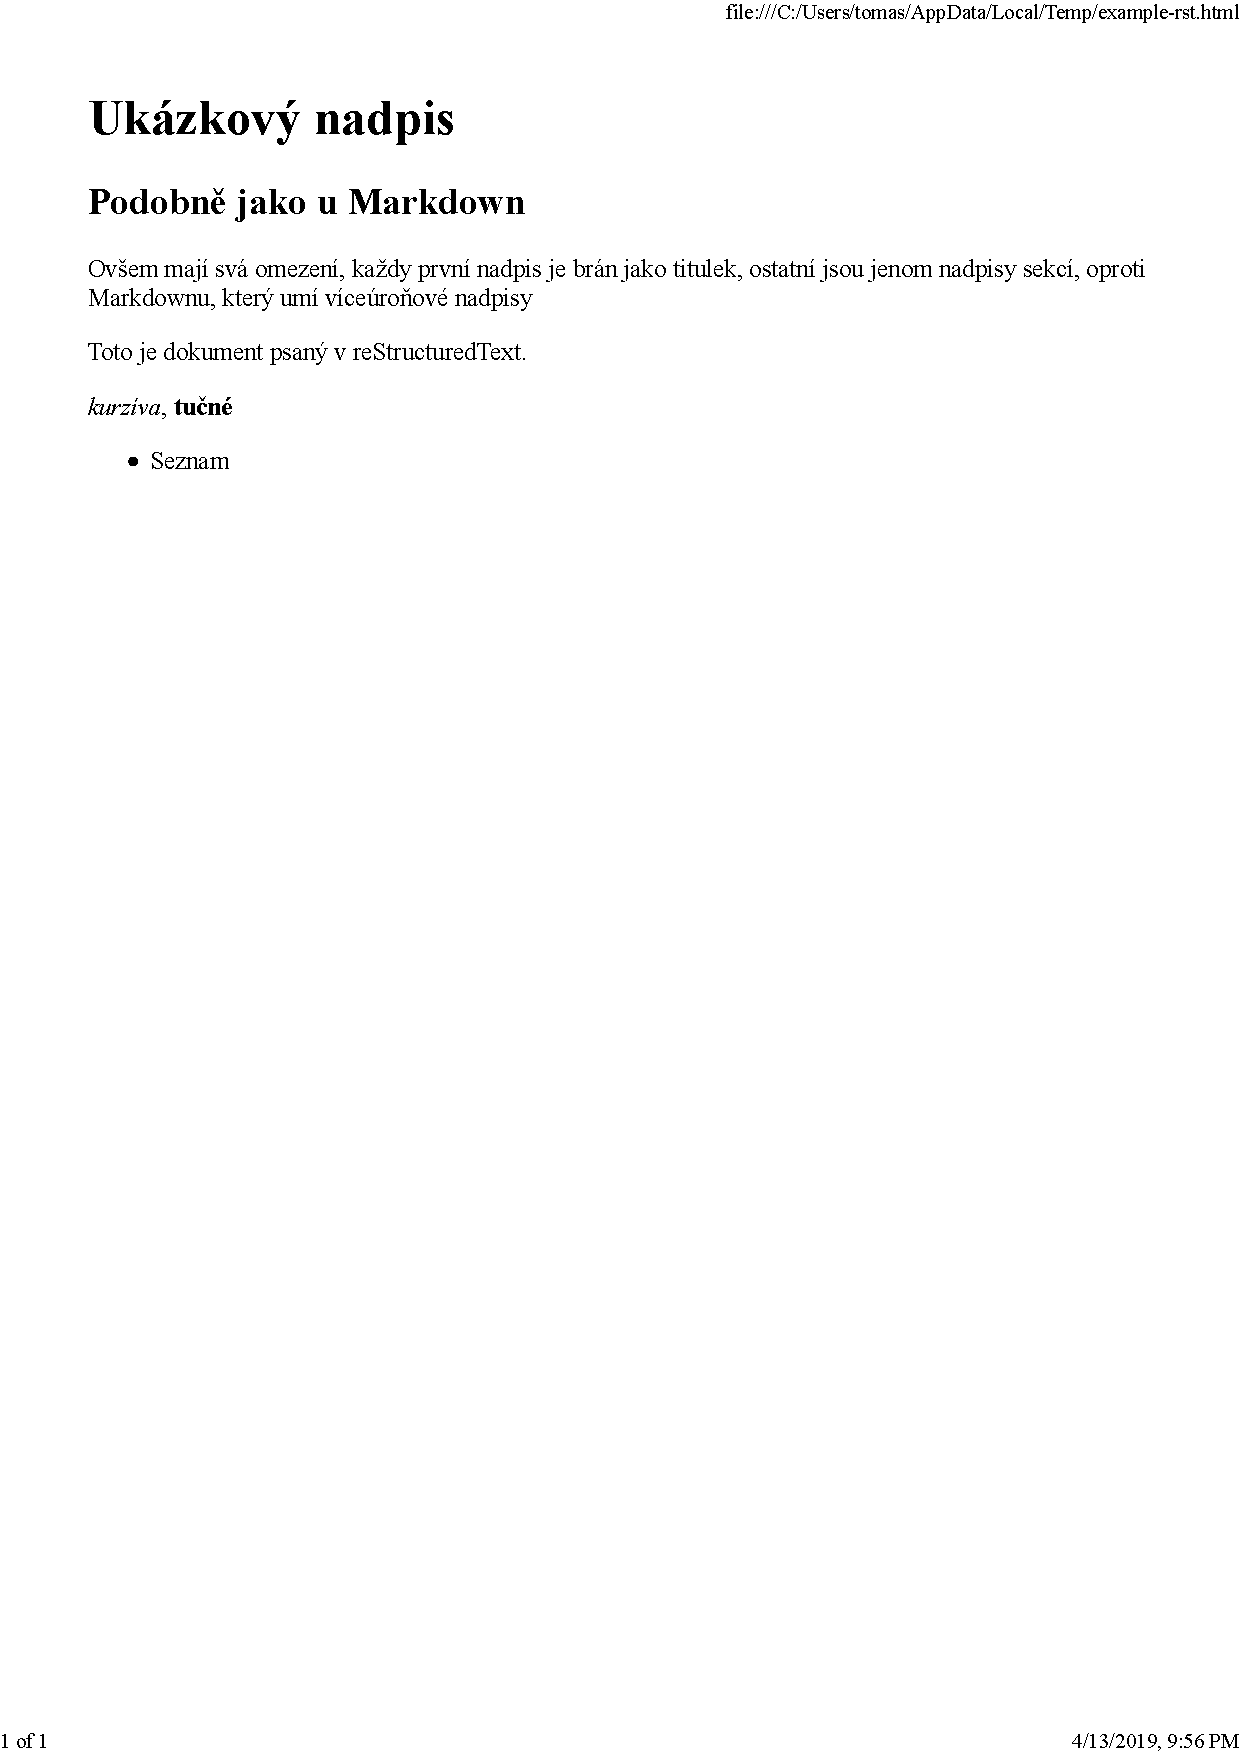
\includepdf{example-rst.pdf}

\section{AsciiDoc}

AsciiDoc je další formát pro psaní dokumentu, jedná se stejně jako reStructuredText, o modul pro jazyk Python. Tento modul je možné použít pro psaní nejenom poznámek,
ale je možné jej exportovat i do formátů jako jsou .epub (formát pro elektronické čtečky knih), či PDF. \cite{asciDoc}